\documentclass[12pt,a4paper]{article}
\usepackage[utf8]{inputenc}
\usepackage[T1]{fontenc}
\usepackage[french]{babel}
\usepackage{amsmath, amssymb, amsfonts}
\usepackage{graphicx}
\usepackage{geometry}
\usepackage{hyperref}
\usepackage{fancyhdr}
\usepackage{setspace}
\usepackage{lmodern}
\usepackage{csquotes}

\geometry{margin=2.5cm}
\pagestyle{fancy}
\fancyhf{}
\rhead{\thepage}
\lhead{Théorie de la spéculation – thèse de Louis Bachelier (1900)}

\usepackage{titling}
\renewcommand\maketitlehooka{\null\mbox{}\vfill}
\renewcommand\maketitlehookd{\vfill\null}

\title{\Huge{\textbf{Théorie de la spéculation\\ Louis Bachelier (1900)}}\\ \medskip
      \Huge{\textit{Article résumé}}\vspace*{0.7cm}}
\author{\LARGE{Alexis VO}\vspace{1cm}\\ \medskip
      Université Paris-Saclay\\École polytechnique}
\date{\vspace{0.2cm}\today}

% === BEGIN DOCUMENT ===
\begin{document}

\vspace{\fill}
  \maketitle
\vspace{\fill}

\newpage

\tableofcontents

\begin{abstract}
En 1900, Louis Bachelier soutient une thèse qui donnera par la suite les bases d’une approche probabiliste des marchés financiers : \textit{La théorie de la spéculation}. Je vous propose dans cet article un résumé après une lecture approfondie de ce texte fondateur. Il s'inscrit dans le cadre de mon stage ayant pour sujet le \textit{Modèle de Cox Ross Rubinstein}. Nous évoquerons les idées de ce mathématicien novateur dans leur contexte historique, en analysant ses modèles mathématiques, et en mettant en lumière leur influence sur la finance moderne. Enfin, nous présenterons les concepts de cours vrai, de prime, d’option et d’équation de la diffusion à travers la modélisation proposée par Bachelier.
\end{abstract}

\newpage

\section{Introduction générale}

\subsection{Contexte historique}

Au tournant du XX\textsuperscript{e} siècle, les marchés financiers comme la Bourse de Paris, connaissent une forte expansion. Les opérations de spéculation y sont nombreuses, mais leur analyse reste essentiellement empirique et intuitive. À cette époque, la probabilité est encore principalement appliquée aux jeux de hasard. Nul ne l'imagine l’appliquer aux mouvements financiers, considérés encore comme trop chaotiques.

C’est dans ce contexte que Louis Bachelier, jeune mathématicien français, propose en 1900 une thèse intitulée \textit{Théorie de la spéculation}. Il modélise mathématiquement les fluctuations boursières en utilisant le calcul des probabilités. Il devient alors le fondateur des mathématiques financières.

\subsection{Présentation de Louis Bachelier}

Louis Bachelier (1870–1946) est un mathématicien français formé à la Sorbonne et élève de Paul Appell. Sa thèse est novatrice à bien des égards : elle est la première à proposer une modélisation stochastique du marché financier. Bien qu’initialement peu reconnue, son œuvre sera redécouverte au XX\textsuperscript{e} siècle, notamment par les économistes et mathématiciens anglo-saxons.

Il est aujourd’hui considéré comme un précurseur de la finance quantitative et un pionnier du mouvement brownien en mathématiques.

\subsection{Objectifs de l'article}

Le présent article propose un résumé d'une lecture active et structurée de la thèse de Bachelier (66 pages). Il vise tout d'abord à présenter les idées clés de la \textit{Théorie de la spéculation} dans un langage accessible aux étudiants de licence. Nous y expliquerons notamment les modèles mathématiques introduits (cours vrai, loi de probabilité, diffusion, etc.) et nous conclurons par la mise en lumière les liens entre les intuitions de Bachelier et les développements ultérieurs en finance moderne.

\subsection{Principales contributions de la thèse}

Dans sa thèse, Bachelier introduit plusieurs concepts fondamentaux. Il modélise dans un premier temps les variations de cours comme un phénomène aléatoire, posant les bases du mouvement brownien avant même Einstein ! Il établit ensuite une loi de probabilité pour les fluctuations de marché, inspirée de la loi normale de Gauss. D'autre part, il formalise des notions toujours utilisées aujourd’hui comme le cours « vrai », les primes, et les options. enfin, il énonce que, dans un marché équilibré, l’espérance mathématique du spéculateur est nulle, anticipant ainsi le \textit{principe d’absence d’arbitrage}.

Ces apports font de sa thèse un texte visionnaire, fondateur de la finance moderne, bien avant l’avènement de modèles comme celui de Black-Scholes.

\section{La Bourse et ses mécanismes au XIX\textsuperscript{e} siècle}

\subsection{Les opérations de Bourse}

Dans les premières pages de sa thèse, Bachelier commence par rappeler les différents types d'opérations que l’on rencontre à la Bourse de Paris, structurées principalement autour des \textit{opérations à terme} :

\begin{itemize}
  \item Les \textit{opérations fermes} : engagements irrévocables d'achat ou de vente à une date future ;
  \item Les \textit{opérations à prime} : options donnant le droit, mais non l'obligation, d’acheter ou de vendre.
\end{itemize}

Il note que ces opérations peuvent se combiner de manière très variée, notamment dans le cas de primes multiples. Cette structuration montre que le marché de l’époque n’est pas seulement un lieu de transaction comptant i.e. un lieu où le réglement ne s'effectue pas seulement à l'achat, mais aussi un lieu de spéculation sur l’évolution future des cours.

\subsection{Opérations fermes et opérations à prime}

Les opérations fermes s’apparentent à des ventes classiques, mais décalées dans le temps. À la liquidation -- qui a lieu en fin de mois -- seule la différence de cours est réglée. Le \textit{cours de compensation} est alors utilisé pour solder les positions. Par exemple, un achat ferme donne un gain si le prix de vente est supérieur au prix d’achat, et une perte dans le cas contraire.

Quant aux opérations à prime, elles ressemblent aux options actuelles :
\begin{itemize}
  \item L’acheteur de la prime paie un montant fixe (la prime) pour bénéficier d’un gain potentiel en cas de hausse (prime à la hausse) ou de baisse (prime à la baisse).
  \item Sa perte est limitée à la prime versée, tandis que son gain est théoriquement illimité.
  \item Le vendeur de prime, à l’inverse, perçoit une prime fixe mais s’expose à une perte potentielle importante.
\end{itemize}
C'est typiquement ce que l'on appelle les options d'achat et de vente (call/put).\\
Bachelier illustre ces opérations par des représentations géométriques (p.~25–26), où l'on peut observer les bénéfices en fonction des cours.

\subsection{Reports, coupons et cours de compensation}

Le \textit{report} est une opération financière qui permet à un acheteur à terme de prolonger sa position au mois suivant. Il paie alors un intérêt au vendeur, sauf cas exceptionnel où cet intérêt est négatif, appelé \textit{déport}.

Sur les valeurs à revenu fixe comme la rente 3~\% de l’époque, les acheteurs perçoivent des \textit{coupons trimestriels}, ce qui crée une asymétrie. D'une part l’acheteur touche les coupons mais paie le report. D'autre part, le vendeur touche le report mais doit verser les coupons.

Bachelier note que cette situation peut générer un avantage pour certaines positions à long terme, comme les \textit{rentes reportables}, où l’achat et le report prolongé sont utilisés pour capter le rendement du coupon.

Le \textit{cours de compensation} est le prix de référence utilisé lors de la liquidation pour évaluer les gains ou pertes. Il est crucial dans la détermination des résultats des opérations à terme.

\subsection{Cours vrai et cours équivalent}

Bachelier introduit la notion essentielle de \textit{cours vrai}. Selon lui, le cours coté sur le marché n’est pas nécessairement le plus juste. Il propose de corriger ce cours en tenant compte des intérêts liés aux coupons à venir, des effets du report, et de la date de liquidation.

Il définit alors des \textit{cours équivalents} comme des prix futurs attendus, ajustés pour refléter la position dans le mois. Par exemple, une rente de 100 francs avec un coupon attendu fera logiquement monter le cours de 0{,}25 franc par mois.

La \textit{courbe des cours vrais} est présentée comme une droite ou une fonction linéaire entre deux liquidations. Cette courbe est centrale pour déterminer la \textit{valeur actualisée} des positions.

Enfin, Bachelier insiste sur l'importance de cette correction car elle permet de calculer des espérances mathématiques équitables. C'est la base de son raisonnement probabiliste.

\bigskip

\noindent
Ainsi, au terme de cette première partie, nous avons  posé les bases de la thèse de Bachelier. Un marché organisé autour d’opérations structurées, une dynamique temporelle claire, et l’introduction d'un point de vue mathématique du comportement des cours. Dans la suite, le mathématicien novateur utilise ces outils pour bâtir un modèle probabiliste rigoureux de la spéculation.

\section{Modélisation mathématique des opérations}

\subsection{Achat, vente et prime}

Comme évoqué précédemment, les \textit{primes} sont l’ancêtre direct des options. Elles sont modélisées comme une combinaison asymétrique d’exposition au risque. L’\textit{achat à prime} donne un bénéfice croissant au-delà d’un certain seuil i.e. le \textit{pied de la prime}, mais limite la perte à la prime versée. La représentation graphique est une droite horizontale (perte fixe) en dessous du seuil, et une pente $+1$ au-dessus.

La figure proposée par Bachelier (fig.~4, p.~30) illustre cela : une \textit{ligne brisée} dont le point de rupture correspond au seuil de rentabilité.

\begin{center}
    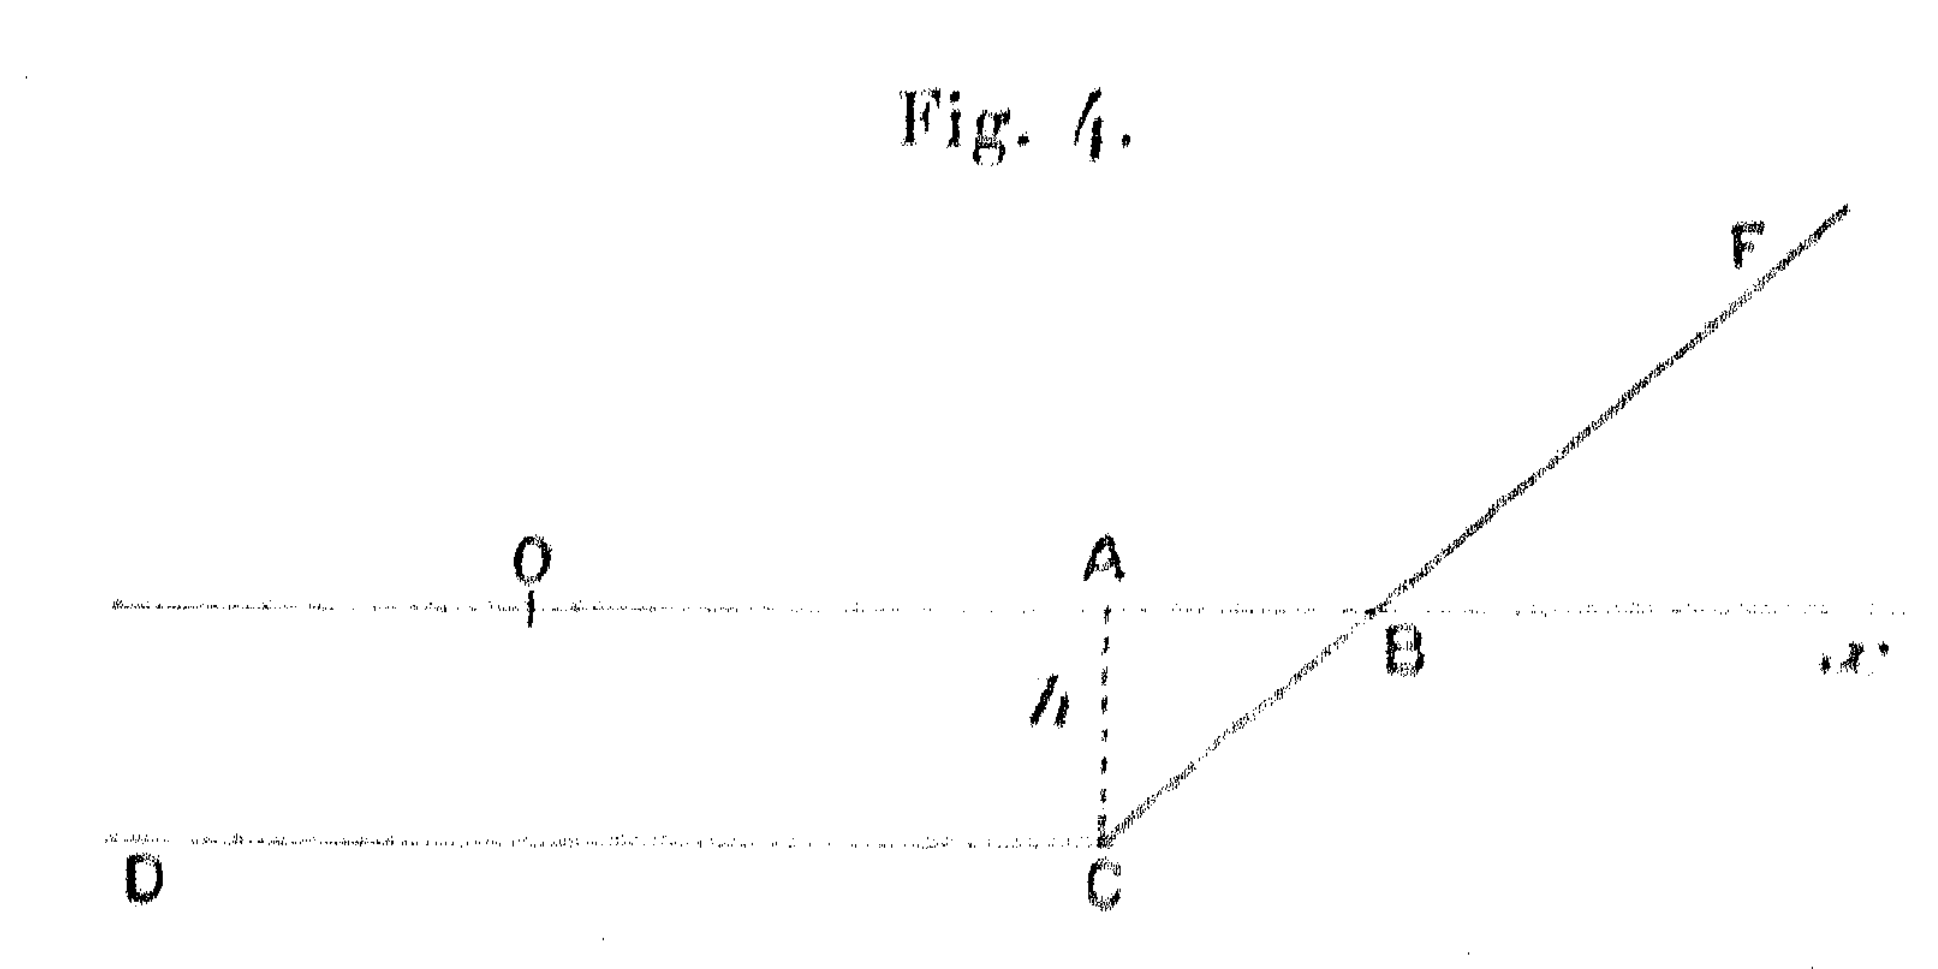
\includegraphics[width=0.5\textwidth]{fig4.png}
\end{center}

Inversement, une \textit{vente à prime} est représentée par une droite brisée en pente négative au-delà du seuil, et plate (gain constant) en dessous. Le vendeur gagne la prime si le marché ne dépasse pas un certain niveau, mais perd au-delà.

Bachelier insiste sur le fait que les marchés à prime permettent de \textit{limiter les pertes}, ce qui les rend attractifs pour certains spéculateurs. Mais cela a un coût ! L'espérance mathématique de la prime est construite de manière à maintenir une neutralité statistique. Il revient sur ce principe plus loin dans sa thèse.

\subsection{Options et stellage}

En complément des opérations simples, Bachelier introduit (p.~31) ce qu’il appelle des \textit{options} (au sens moderne du terme), c’est-à-dire des instruments hybrides entre le ferme et la prime.

Il donne l’exemple d’une \textit{option du double} : une position qui donne droit à deux unités de gain en cas de hausse, mais seulement à une unité de perte en cas de baisse. On parle aujourd’hui d’option asymétrique. De telles structures permettent de moduler le profil de risque selon les anticipations.

De plus, il décrit le \textit{stellage} -- ou \textit{double prime} -- constitué d’une prime à la hausse combinée avec une prime à la baisse. On l’interprète aujourd’hui comme une \textit{stratégie de tunnel, appelée straddle}.

Ce montage donne :
\begin{itemize}
  \item un gain si le cours s’éloigne significativement du cours d’exercice i.e. volatilité grande,
  \item une perte limitée à la somme des deux primes si le cours reste stable.
\end{itemize}

Le stellage est donc une \textit{stratégie directionnellement neutre}, qui mise uniquement sur l’ampleur des mouvements, et non leur sens.

\bigskip

\noindent
Au terme de cette seconde partie, nous avons compris que cette modélisation des opérations financières est l’un des apports pédagogiques majeurs de Bachelier. Elle permet de visualiser les profils de gains et pertes associés à chaque type d’opération, et prépare le terrain à une analyse probabiliste des stratégies, développée dans les sections suivantes.

\section{Probabilités dans les opérations financières}
\subsection{Probabilités mathématiques et spéculatives}
\subsection{Espérance mathématique et équité du marché}
\subsection{Avantage mathématique}

\section{La dynamique des cours}
\subsection{Loi de probabilité des cours}
\subsection{Équation de diffusion (équation de Fourier)}
\subsection{Solution gaussienne}
\subsection{Écart-type et espérance en fonction du temps}

\section{Applications aux options et primes}
\subsection{Prime simple : calcul et probabilité de réussite}
\subsection{Écart probable et valeur attendue}
\subsection{Double prime et loi des écarts}
\subsection{Formule intégrale et interprétations}

\section{Vision moderne du modèle de Bachelier}
\subsection{Comparaison avec le modèle de Black-Scholes}
\subsection{Limites du modèle de Bachelier}
\subsection{Malentendus et critiques}

\section{Héritage et influence}
\subsection{Pourquoi Bachelier fut ignoré}
\subsection{Réhabilitation au XX\textsuperscript{e} siècle}
\subsection{Impact sur la finance quantitative moderne}

\section{Conclusion}
\subsection{Synthèse mathématique}
\subsection{Apports théoriques et historiques}
\subsection{Perspectives actuelles}

\appendix
\section*{Annexes}
\addcontentsline{toc}{section}{Annexes}
\subsection*{A. Reproduction de figures de la thèse}
\subsection*{B. Détails de formules mathématiques}
\subsection*{C. Références bibliographiques}
\subsection*{D. Glossaire des termes techniques}

\end{document}